\documentclass{acm_proc_article-sp}

\usepackage[utf8]{inputenc}
\usepackage[brazil]{babel}
\usepackage{graphicx}
\usepackage[lined,boxed,commentsnumbered]{algorithm2e}
\usepackage[normalem]{ulem}
%\usepackage{algorithm2e}
%\usepackage{draftwatermark}
% path to spreadsheet with test data and graphs: "Google Drive\Doutorado\Pesquisa\Testes\WsnEE\"
% file name: "WsneeFD - Experimental Data + Grafs - 1000 Cycles - Averages (Fernando) - 19082014.ods"
% sub-path to graphic files: "Gráficos\Gráficos BCWSN SD=1 CD=5"
% path to files for upload project: "Google Drive\Doutorado\Pesquisa\Artigos\SAC2015\SACLatex"


% correct bad hyphenation here
\hyphenation{op-tical net-works semi-conduc-tor sche-dul-ing}
\newcommand{\dia}{\hspace*{.1cm} \hfill $\diamond$}


\begin{document}

\title{Usando Agrupamento Fractal para explorar Correlação Comportamental: Uma nova
abordagem para reduzir o consumo de energia em RSSF}

% \title{Using Fractal Clustering to explore Behavioral Correlation: A new
% approach to reduce energy consumption in WSN}

% author names and affiliations
% use a multiple column layout for up to three different
% affiliations
% \author{\IEEEauthorblockN{Fernando Rodrigues}
% \IEEEauthorblockA{University of Fortaleza\\Fortaleza - Ceara - Brazil\\
% fernandorodrigues@edu.unifor.br}
% \and
% \IEEEauthorblockN{Angelo Brayner}
% \IEEEauthorblockA{University of Fortaleza\\
% Fortaleza - Ceara - Brazil\\
% brayner@unifor.br}
% \and
% \IEEEauthorblockN{Jose E. Bessa Maia}
% \IEEEauthorblockA{State University of Ceara\\
% Fortaleza - Ceara - Brazil\\
% jose.maia@uece.br}}



% make the title area
\maketitle


\begin{abstract}

Agrupamento de sensores é uma estratégia eficaz para reduzir o número de
mensagens sendo transmitidas em uma rede de sensores sem fio (RSSF) e assim,
reduzir o consumo de energia. Este artigo apresenta uma nova abordagem para
agrupamento de sensores em redes de sensores, chamado Correlação Comportamental
em RSSF (BCWSN, da sigla em inglês), que se baseia no comportamento de dados
recentes coletados pelos sensores. Em vez de usar a distância espacial entre os
sensores, a abordagem proposta inicializa clusters usando os conceitos de
similaridade na magnitude e tendência de dados de sensoriamento.
Para a manutenção dos clusters, o BCWSN implementa o conceito de Agrupamento
Fractal (ou Fractal Clustering) para encontrar, dinamicamente, a melhor forma
para a configuração dos clusters. A fim de validar nossa abordagem, simulações
foram realizandas sobre dados reais.
Os resultados mostram que o BCWSN pode reduzir o número de mensagens injetadas
na rede em até $94,80\%$ em relação a uma abordagem naive (sem agrupamento, sem
predição e sem supressão) e até $57,24\%$ quando comparado com abordagens
implementando correlação temporal, enquanto o Erro Quadrático Médio (EQM)
permanece praticamente estável.


% Sensor clustering is an efficient strategy to reduce the number of messages
% flowing in a Wireless Sensor Network (WSN) and thereby reducing the energy
% consumption. This paper presents a new approach to cluster sensors in WSNs,
% called Behavioral Correlation in WSN (BCWSN), which is based on the behavior of
% recent historical data collected by sensors. Instead of using spatial distance
% among sensors, the proposed approach initializes clusters using the concepts of
% similarity in magnitude and trend of sensed data. For clusters maintenance,
% BCWSN implements the notion of Fractal Clustering to dynamically find the best
% configuration for clusters. In order to validate our approach, simulations have
% been conducted over real data. The results show that BCWSN can reduce the number
% of messages injected into the network up to 94.80\% over a naive approach (no
% clustering, no prediction and no suppression) and up to 57.24\% when compared to
% approaches implementing temporal correlation, while RMSE remains roughly stable.

\end{abstract}

% \category{H.2.m}{Database Management}{Miscellaneous}
% 
% \terms{Algorithms, Measurement, Performance}
% 
% % keywords
% \keywords{Wireless sensor networks, Behavioral correlation, Fractal clustering, 
% Temporal correlation, Energy efficiency}




\section{Introdução}
% no \IEEEPARstart

Os avanços na tecnologia de redes sem fio permitiram o desenvolvimento de redes
de sensores sem fio (RSSF) em grande escala. Nós sensores são dispositivos
utilizados para medir fenômenos físicos ambientais. Eles são limitados em
potência, capacidade computacional e de memória. Numa RSSF, os sensores são
geralmente dispersos na rede e usam canais de comunicação de baixa potência para
disseminar dados coletados para uma estação base. Devido a estas
características, RSSF têm sido amplamente utilizadas para o monitoramento
ambiental (por exemplo, habitat), sensoriamento industrial e diagnósticos (por
exemplo, fábricas e cadeias de abastecimento), proteção de infra-estruturas (por
exemplo, distribuição de água), reconhecimento de campo de batalha (por exemplo,
direcionamento multi-alvo) e aplicações de computação ubíqua (por exemplo, casas
inteligentes) \cite{MaiaACR2013}.
% Advances in wireless technology have enabled the development of massive-scale
% wireless sensor networks (WSNs). Sensors nodes are devices used to measure
% physical phenomena from the environment. They are limited in power,
% computational capacity, and memory. In a WSN, sensors are usually scattered in
% the network and use low-power communication channels to disseminate collected
% data to a base station. Due to these characteristics, WSNs have been widely used
% for environmental monitoring (e.g., habitat), industrial sensing and diagnostics
% (e.g., factory, supply chains), infrastructure protection (e.g., water
% distribution), battlefield awareness (e.g., multi-target tracking) and
% context-aware computing (e.g., intelligent home) applications
% \cite{MaiaACR2013}.
\vspace*{-.3cm}

Apesar dos avanços na tecnologia de RSSF, um ponto-chave ainda é o consumo de
energia dos nós sensores. Na verdade, a comunicação entre os sensores é, de
longe, a atividade que consome mais energia em uma WSN.
Ao reduzir custos de comunicação, a energia total pode ser drasticamente
economizada, consequentemente aumentando a vida útil da RSSF. Uma estratégia
eficaz para reduzir o consumo de energia é, por isso, reduzir o número de
mensagens enviadas através da rede.
No entanto, quanto menor o número de dados sensoriados que for transmitido,
menor a precisão dos resultados fornecidos por uma RSSF. Assim, uma maior
precisão em RSSF vem com um maior custo energético.
% In spite of advances in WSN technology, a critical key point is still energy
% consumption of sensor nodes. As a matter of fact, communication among sensors is
% by far the activity which consumes more energy in a WSN. By reducing
% communication costs, energy power may be drastically saved, consequently
% increasing WSN's lifetime. An effective strategy to reduce energy consumption
% is, therefore, to reduce the number of messages sent across the network.
% Nevertheless, the less the number of sensed data is transmitted, the lower the
% accuracy of results provided by a WSN. Thus, higher accuracy in WSNs comes at a
% higher energy cost.
\vspace*{-.3cm}

Agrupamento de nós sensores numa RSSF pode reduzir o número de mensagens que são
transmitidas na RSSF. Isto acontece porque os Cluster Heads, os quais são
responsáveis por um grupo de nós sensores, coordenam o fluxo de dados
(mensagens) entre os sensores e o sink. Ao fazer isso, o Cluster Head (CH) manda
apenas mensagens ``importantes'' para o sink. Várias abordagens têm sido
implementadas para formar agrupamentos em RSSF, onde a maioria delas são
baseados na correlação espacial dos sensores da RSSF.
% Clustering sensor nodes in a WSN may reduce the number of messages flowing in a
% WSN. This is because Cluster Heads, which are responsible for a set of sensor
% nodes, coordinate the data flow (messaging) between sensors and the sink.
% By doing that, the Cluster Head (CH) forward to the sink node ``important''
% messages. Several approaches have been implemented to form clusters in WSNs,
% where most of them are based on spatial correlation of the data sensors of the
% WSN.
\vspace*{-.3cm}

Até agora, sabe-se bem que os dados coletados pelas redes de sensores são
espacialmente ou temporalmente correlacionados \cite {Chu2006, Villas2012,
Yoon2005}. A correlação temporal afirma que é muito provável que as leituras
detectadas num pequeno intervalo de tempo de um determinado nó sensor têm muitos
valores aproximados (localidade temporal). Esta propriedade torna possível
predizer (com um determinado limiar de erro) futuros valores coletados com base
em dados coletadas no passado. Por outro lado, a correlação espacial de dados
está relacionada com a idéia de que a proximidade física entre os sensores pode
levar a medições semelhantes dos dados (localidade espacial).
Assim, é possível estimar os valores detectados por sensores em uma região R com
base nas leituras de um sensor S localizado na mesma região R.
% So far, it is well known that data collected by WSNs are spatially or temporally
% correlated \cite{Chu2006, Villas2012, Yoon2005}. Temporal correlation states
% that it is very likely that readings sensed in a lapse of time by a given node
% have very nearly values (temporal locality). This property makes possible to
% predict (with a given error threshold) future sensed values based on data
% collected in the past. On the other hand, spatial data correlation is related to
% the idea that physical proximity among sensors may lead to similar measurements
% of sensed data (spatial locality). Thus, it is possible to estimate values
% sensed by sensors in a region R based on the readings of a sensor S located in R
% as well.
\vspace*{-.3cm}

No entanto, em várias situações, sensores que não estão espacialmente próximos
uns aos outros podem também ter padrões de leitura de dados semelhantes.
A fim de ilustrar esta afirmação, considere uma RSSF densa implantada para
monitorar incêndios florestais. Agora, suponha um cenário em que a região
monitorada é afetada por dezenas de pequenos incêndios florestais.
A Figura \ref{fig:contour_lines} retrata possíveis ``curvas de nível'' de
temperatura para esta situação. Observe na Figura \ref{fig:contour_lines} que há
várias regiões fechadas, que representam campos com áreas de incêndios
florestais. As medições de temperatura detectadas pelos sensores naqueles
regiões espacialmente separadas podem apresentar alta correlação.
Em tais casos, as técnicas de correlação de dados espaciais tradicionais,
utilizando a distância física entre os sensores, não são eficientes para
detectar correlação espacial. Consequentemente, aquelas técnicas não são
adequadas para serem aplicadas como critério para agrupar os sensores em uma
RSSF.
% However, in several scenarios, sensors which are not spatially close to each
% other may also have similar data reading patterns. In order to illustrate this
% statement, consider a dense WSN deployed to monitor forest fires.
% Now, suppose a scenario in which the monitored region is affected by dozens of
% small forest fires. Figure \ref{fig:contour_lines} depicts possible temperature
% contour lines for this situation. Observe in Figure \ref{fig:contour_lines} that
% there are several closed regions, which represents fields with forest fire areas.
% The temperature measurements sensed by sensors in those spatially separated
% regions may present high correlation. In such cases, traditional spatial data
% correlation techniques, using physical distance among sensors, are not efficient
% to detect spatial correlation. Consequently, it is not adequate for being
% applied as a criterion to cluster sensors in a WSN.

\begin{figure}[!htb]
\centering
	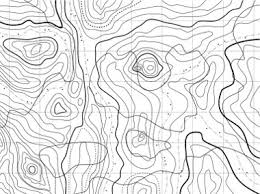
\includegraphics[scale=0.8]{I2.png}
    \caption{Linhas de Contorno da Temperatura}
    \label{fig:contour_lines}
\end{figure}
\vspace*{-.3cm}

Por isso, propomos uma nova abordagem para a detecção de correlação de dados
entre os dados produzidos por uma RSSF, baseado no conceito de {\it correlação
comportamental}. O principal objetivo da abordagem proposta, chamada {\it
Correlação Comportamental em RSSF} (BCWSN), é identificar padrões similares de
leituras de dados, a fim de agrupar os sensores dinamicamente, com o número
mínimo de mensagens trocadas, mesmo quando os sensores estão geograficamente
distantes uns dos outros. Neste sentido, propomos a utilização da noção de {\it
Agrupamento Fractal} (ou {\it Fractal Clustering}) \cite{Barbara2000}, que pode
fazer a manutenção dos clusters no sink exatamente quando ``novidades'' são
recebidas, sem necessidade de mais leituras de dados de outros sensores do mesmo
cluster.
No entanto, {\it Agrupamento Fractal} é uma técnica de agrupamento incremental
utilizando o cálculo da Dimensão Fractal, e, consequentemente, ela é incapaz de
inicializar o agrupamento de sensores desde o início, requerendo uma formação
inicial dos agrupamentos (ou clusters). Desta forma, a correlação comportamental
é calculado inicialmente a partir de séries temporais de leituras de sensores,
aplicando {\it Medidas de Similaridade}, semelhantes as encontradas em
\cite{Liu2007}. Assim, a Correlação Comportamental é capaz de capturar a
similaridade na magnitude e na tendência nos dados obtidos.
% For that reason, we propose a new approach for detecting data correlation among
% data produced by a WSN, based on the concept of {\it behavioral correlation}.
% The main goal of the proposed approach, called  {\it Behavioral Correlation in
% WSN} (BCWSN), is to identify similar patterns of data readings in order to
% dynamically cluster sensors, with the minimal number of messages exchanged, even
% when sensors are geographically distant from each other. In this sense, we
% propose to use the notion of {\it Fractal Clustering} \cite{Barbara2000}, which
% can make clusters maintenance in sink just when ``novelties'' are received,
% without need of more data readings from other sensors in the same cluster.
% However, {\it Fractal Clustering} is an incremental clustering technique using
% the Fractal Dimension calculation, hence it is unable to initialize sensor
% clusters from the beginning, requiring an initial cluster formation. This way,
% behavioral correlation is computed initially from the time series of sensor
% readings by applying {\it Similarity Measure} \cite{Liu2007}.
% Thus, Behavioral Correlation is able to capture similarity in magnitude and
% trend of sensed data.
\vspace*{-.3cm}

% Thus, Behavioral Correlation is able to capture similarity in magnitude and
% trend of sensed data instead of using spatial distance among sensors for
% identifying correlation among data.

% Based on the concept of Behavioral Correlation, this paper presents a new
% approach for clustering sensors in WSNs, called Behavioral Correlation in WSN
% (BCWSN). 

A idéia é aplicar o BCWSN para inicialização (usando {\it Medidas de
Similaridade}) e manutenção (usando {\it Agrupamento Fractal}) da melhor
configuração de agrupamentos em uma RSSF.
% The idea is to apply BCWSN for initializing (using {\it Similarity Measure}) and
% maintaining (using {\it Fractal Clustering}) the best cluster configuration in a
% WSN.
\vspace*{-.3cm}

% Behavioral correlation may vary in time, which can in turn impose modification
% on the initial cluster configuration. Thus, for clusters maintenance, BCWSN
% implements the notion of Fractal Dimension to dynamically find the best
% configuration for clusters. The idea is to apply fractal dimension to verify if
% the behavioral correlation computed for defining the initial cluster
% configuration is still valid. This method is triggered whenever new data arrives
% at the sink.
% The sink will analyze, through the Minimum Difference of Fractal Dimension,
% whether such data are just ``noise'' or actually they represent ``novelties''. 
% Nevertheless, in order to avoid that every sensed data be transmitted to the
% sink node, an in-network data prediction model is applied to compute data
% temporal correlation.
% \vspace*{-.3cm}

% For that reason, we propose a new approach for detecting data correlation among
% data produced by a WSN. The main goal of the proposed approach, called  {\it
% Behavioral Correlation}, is to identify similar patterns of sensor readings
% even in sensors geographically distant from each other. Behavioral Correlation
% is computed from the time series of sensor readings by applying {\it
% Similarity Measure} \cite{Liu2007}. This way, Behavioral Correlation is able to
% capture similarity in magnitude and trend of sensed data instead of using
% spatial distance among sensors for identifying correlation among data.
% \vspace*{-.3cm}
% 
% Based on the concept of Behavioral Correlation, this paper presents a new
% approach for clustering sensors in WSNs, called Behavioral Correlation in WSN
% (BCWSN). The idea is to apply behavioral correlation for defining an initial
% cluster configuration in a WSN.
% \vspace*{-.3cm}
% 
% Behavioral correlation may vary in time, which can in turn impose modification
% on the initial cluster configuration. Thus, for clusters maintenance, BCWSN
% implements the notion of Fractal Dimension to dynamically find the best
% configuration for clusters. The idea is to apply fractal dimension to verify if
% the behavioral correlation computed for defining the initial cluster
% configuration is still valid. This method is triggered whenever new data arrives
% at the sink.
% The sink will analyze, through the Minimum Difference of Fractal Dimension,
% whether such data are just ``noise'' or actually they represent ``novelties''. 
% Nevertheless, in order to avoid that every sensed data be transmitted to the
% sink node, an in-network data prediction model is applied to compute data
% temporal correlation.
% \vspace*{-.3cm}

O restante deste documento está organizado da seguinte forma: a Seção 
\ref{related-work} descreve trabalhos relacionados e delineia as diferenças
entre o nosso método e métodos existentes. Na Seção \ref{implementing-bcwsn},
o método de Correlação Comportamental em RSSF (BCWSN) proposto é apresentado e 
discutido. Simulações com um protótipo em Sinalgo \cite{Sinalgo2007} executado
com dados de sensores reais são apresentados e discutidos na Seção \ref{eval}.
Finalmente, a Seção \ref{conclusion} conclui o artigo.
% The remainder of this document is organized as follows: Section
% \ref{related-work} describes related work and outlines the differences between
% our method and existing methods. In Section \ref{implementing-bcwsn}, the
% proposed Behavioral Correlation in WSN (BCWSN) method is presented and
% discussed. Simulations with a Sinalgo \cite{Sinalgo2007} prototype executed over
% real sensor data are presented and discussed in Section \ref{eval}. Finally,
% Section \ref{conclusion} concludes the paper.
\vspace*{-.3cm}

\section{Trabalhos Relacionados}
\label{related-work}

Em EEDC \cite{Liu2007}, medidas de dissimilaridade são calculadas pelo 
nó sink para pares de nós com base em até $3$ parâmetros, a saber: {\it (i)}
diferença de magnitude (\textit{M}) e {\it (ii)} tendência (\textit{T}) dos
valores dos dados e {\it (iii)} distância geográfica / euclidiana entre
os nós ($g_{max}dist$).
O critério de formação de agrupamentos é baseada no limiar máximo de
dissimilaridade (max\_dst) defida por uma tupla (\textit{M}, \textit{T},
$g_{max}dist$). Funciona da seguinte maneira: $1)$ Inicialmente, os dados de
sensoriamento de cada nó são enviados na forma de uma série temporal para o
sink. $2)$ Em seguida, o sink armazena todos os dados dos sensores e então
calcula a medida de dissimilaridade para cada par de nós da rede. $3)$ Com as
medidas calculadas e o limiar máximo de dissimilaridade (max\_dst), o sink
divide os nós em clusters (agrupamentos). Para cada agrupamento, o sink faz
simultaneamente, o agendamento equitativo – round robin - junto com a escolha
aleatória de nós representativos, cujas leituras de dados servem como
representativos para todo o agrupamento. Porém, esse trabalho não leva em conta
a reserva de energia de cada nó como um critério para a escolha de nós
representativos. Neste trabalho, o Cluster Head é escolhido de acordo com o
nível de energia remanescente e a distância mínima para o sink.
Além disso, diferentemente de \cite{Liu2007}, neste trabalho podemos levar em
conta leituras de múltiplos tipos de dados diferentes por sensores.
% In EEDC \cite{Liu2007}, measures of dissimilarity are calculated by the sink
% node for pairs of nodes based on up to $3$ parameters, namely: {\it (i)}
% differences in magnitude (\textit{M}) and {\it (ii)} trend (\textit{T}) of the
% data values and {\it (iii)} geographical/euclidean distance between nodes
% ($g_{max}dist$).
% The criterion of formation of clusters is based on the maximum threshold of
% dissimilarity (max\_dst) defined by a tuple (\textit{M}, \textit{T},
% $g_{max}dist$). It works as follows: $1)$ Initially, the sensed data by each
% node are sent in the form of a temporal series to the sink. $2)$ Then the sink
% stores all the data from the sensors and afterwards calculates the measure of
% dissimilarity for each pair of nodes of the network. $3)$ With the calculated
% measures and the maximum threshold of dissimilarity (max\_dst), the sink divides
% the nodes into clusters. For each cluster, the sink makes, simultaneously, the
% equitable scheduling - round robin - along with the random choice of
% representative nodes, whose data readings will serve as the representatives for
% the whole cluster.
% However, that work does not take into account the energy reserve of each node as
% a criterion for choosing representative nodes. In this work, we chose Cluster
% Heads according to the remaining energy level and the minimum distance to the
% sink. Moreover, unlike \cite{Liu2007}, we can take into account readings from
% multiple different data types by sensors.
\vspace*{-.3cm}

Carvalho \textit{et al.} \cite{Carvalho2011} propôs aplicar uma Correlação
Espaço-Temporal Multivariada para melhorar a precisão da predição em uma RSSF.
No entanto, esse trabalho não reduz o consumo de energia da rede. Na verdade,
ele ainda aumenta o consumo de energia da rede, em muitas situações. Em nosso
trabalho, por meio de regressão linear múltipla com Agrupamento Fractal,
conseguimos a redução do consumo de energia total da rede, obtendo resultados
com um Erro Quadrático Médio (EQM) para a predição de dados (com relação aos
dados coletados) ainda menor do que outras abordagens.
% Carvalho \textit{et al.} \cite{Carvalho2011} proposed applying Multivariate
% Spatio-Temporal Correlation to improving prediction accuracy in a WSN. However,
% that work does not reduce the energy consumption of the network. In fact, it
% even increases the energy consumption of the network in many situations. In our
% work, using multiple linear regression with Fractal Clustering, we achieved the
% reduction of the overall energy consumption of the network, obtaining results
% with a Root Mean Square Error (RMSE) for the prediction data (w.r.t. the sensed
% data) even smaller than other approaches.
\vspace*{-.3cm}

Barbará and Chen \cite{Barbara2000} propuseram um método, chamado {\it Fractal
Clustering} (FC), para agrupar conjuntos de dados.
Nesse trabalho, uma etapa de iniciação baseada na estratégia do vizinho mais
próximo cria os clusters (agrupamentos) iniciais. Em seguida, ele implementa o
algoritmo do passo incremental, que usa o cálculo do \textit{Fractal Dimension}
com base na implementação do algoritmo de \textit{Box Counting}, chamado FD3
\cite{Liebovitch1989}. Em nosso trabalho, uma versão estendida do método FC é
proposta (BCWSN). No nosso caso, o sink usa medida de similaridade (ver Passo 2
na Seção \ref{implementing-bcwsn}) na etapa de iniciação para formar grupos
iniciais. Para manutenção de clusters, nós implementamos um algoritmo de Fractal
Clustering “especial” (ver Passo 5 na Seção \ref{implementing-bcwsn}), que
identifica se a leitura de dados recebidos pelo sink são apenas ``ruído'' ou, na
verdade, eles representam ``novidades'', e evita um grande volume de mensagens
para receber os dados lidos de todos os sensores nos mesmos clusters, uma vez
que o FC precisa apenas de novos dados ``reais'' para funcionar corretamente.
% Barbar\'{a} and Chen \cite{Barbara2000} proposed a method, called {\it Fractal
% Clustering} (FC), to cluster datasets. In that work, an initialization step
% based on the nearest neighbor strategy creates the initial clusters. Then, it
% implements the algorithm of incremental step, which uses \textit{Fractal
% Dimension} calculation based on an implementation of Box Counting algorithm,
% called FD3 \cite{Liebovitch1989}. In our work, an extended version of FC method
% is proposed (BCWSN). In our case, sink uses Similarity Measure (see Step 2 in
% Section \ref{implementing-bcwsn}) in the initialization step to form initial
% clusters. For clusters maintenance, we implemented a ``special'' Fractal
% Clustering algorithm (see Step 5 in Section \ref{implementing-bcwsn}), which
% identifies whether data reading received by sink are just ``noise'' or actually
% they represent ``novelties'', and avoids a bulk of messages to receive the data
% reading of all sensors at same clusters, since FC needs only ``real'' new data
% to work properly.
\vspace*{-.3cm}

% Barbar\'{a} and Chen \cite{Barbara2000} proposed a method, called {\it Fractal
% Clustering} (FC), to cluster datasets. In that work, an initialization step
% based on the nearest neighbor strategy creates the initial clusters. Then, it
% implements the algorithm of incremental step, which uses \textit{Fractal
% Dimension} calculation based on an implementation of Box Counting algorithm,
% called FD3 \cite{Liebovitch1989}. In our work, an extended version of FC
% method is proposed (BCWSN). In our case, sink uses Similarity
% Measure (see Step 2 in Section \ref{implementing-bcwsn}) in the initialization
% step to form initial clusters. \sout{An in-network data prediction strategy is used in
% order to avoid that every sensed data be transmitted to the sink node.} \sout{However,
% Behavioral Correlation may vary in time at some sensed regions. For that
% reason, new data can arrive at the sink.} Thus, we implemented a ``special''
% Fractal Clustering algorithm (see Step 5 in Section \ref{implementing-bcwsn})
% for clusters maintenance, which avoids a bulk of messages to receive the data
% reading of all sensors \sout{from the same involved clusters, since FC needs only
% ``real'' new data}.

Adaga-P* \cite{MaiaACR2013} constrói modelos de campos de sensores que
implicitamente implementam correlação espacial para agrupar sensores.
Além do mais, ele define e usa um modelo de predição de dados em rede para
reduzir o número de mensagens injetadas na rede. Não obstante o acima exposto,
ele não é capaz de agrupar os sensores baseados no comportamento dos dados dos
sensores (ou ``padrão de dados de leitura''). Assim, em algumas situações, o
BCWSN agrupa sensores de uma forma mais otimizada, reduzindo o tráfego de
mensagens da rede.
% Adaga-P* \cite{MaiaACR2013} constructs sensor-field models which implicitly
% implements spatial correlation to cluster sensors. Furthermore, it defines and
% uses an in-network data prediction model to reduce the number of messages
% injected into the network. Notwithstanding the above, it is unable to cluster
% sensors based on the behavior of sensor data (or ``data reading pattern'').
% Thus, in some situations, BCWSN groups sensors in a more optimized way, reducing
% the message traffic on the network.
\vspace*{-.3cm}

\section{Implementando Correlação Comportamental em RSSFs}
\label{implementing-bcwsn}

%\\PAREI AQUI!!


A fim de construir uma configuração de cluster inicial, BCWSN implementa
a ideia dissimilaridade de Medida, que é responsável pela correlação
comportamental informática. Correlação comportamental pode variar no tempo,
o que por sua vez pode impor modificação na configuração do cluster inicial.
Por essa razão, BCWSN implementa o conceito de Fractal Clustering
\cite{Barbara2000}. Em nossa proposta,uma rede de sensores consiste
em um sink node (a.k.a. estação de base ou centro de fusão) e um conjunto
de nós sensores dispersos em uma região.
Assim, sempre que novos dados chegam ao sink, ele analisa-os através do método
de diferença mínima para a Fractal Dimension (descrito abaixo) para
identificar se esses dados são apenas ``ruído'' ou ``novidades''. 
Se o valor de diferença mínima para Fractal Dimension(valor do MDFD)
está acima um certo limite,($\sigma$) ou se um número máximo de ``ruído'' 
para uma nó sensor dado é atingido. Então, ele irá acionará um processo de
divisão do cluster. Caso contrário, se o valor de MDFD for superior a um 
limiar de ruído($\tau$), a quantidade de ``ruído'' para o nó sensor é 
incrementado. Caso contrário, o nó sensor(que enviou os ``novidades'')
será mudou-se para o cluster escolhido, ou seja, aquele que tem uma pequena
diferença em será transferido para o cluster escolhido, ou seja, aquele que
tem uma menor diferença na dimensão fractal com a inclusão de novos dados.
% In order to build an initial cluster configuration, BCWSN implements the idea of
% Similarity Measure, which is responsible for computing Behavioral Correlation.
% Behavioral Correlation may vary in time, which can in turn impose modification
% on the initial cluster configuration. For that reason, BCWSN also implements the
% concept of Fractal Clustering \cite{Barbara2000}. In our proposal, a sensor
% network consists of a sink node (a.k.a. base station or fusion center) and a set
% of sensor nodes scattered in a region.
% Thus, whenever new data arrive at the sink, it analyzes them, through the
% Minimum Difference of Fractal Dimension method (described below) for identifying
% if such data are just ``noise'' or ``novelties''. If the value of Minimum
% Difference of Fractal Dimension (MDFD value) is above a certain split threshold
% ($\sigma$) or a maximum number of ``noise'' for a given sensor node is reached,
% then it will trigger a split process. Else, if the MDFD value is above a noise
% threshold ($\tau$), the number of ``noise'' for that sensor node is
% incremented. Otherwise, the sensor node (which sent the ``novelties'') will be
% relocated to the chosen cluster, i.e., one that has a smaller difference in
% Fractal Dimension with the inclusion of new data.
\vspace*{-.3cm}


%\subsection{The BCWSN Mechanism}
BCWSN pode ser dividida em cinco etapas, como descrito a seguir. 
% BCWSN can be divided into five steps as described next.
\vspace*{-.3cm}

%\subsubsection{Learning Stage}
{\bf Step 1 - Learning Stage}
Nesta etapa, o nó sink coleta dados sensoriais de todos os sensores
{pertencentes à rede}, a fim de calcular a formação do aglomerado inicial e os
coeficientes da equação de regressão linear (ver Passo 3). Assim, o nó sorvedouro primeiramente envia uma mensagem de
broadcast para todos os nós da rede, solicitando os seguintes dados de sensores: Nível da bateria,
localização espacial e valores detectados. A quantidade de dados utilizados pela fase de
aprendizagem é um parâmetro, denotada \textit{programação inicial}. A qual
deverá ser definida por uma aplicação expert(Por exemplo 70). Cada sensor responde à mensagem de transmissão
do sink, em lote, ou seja, faz todo sensoriamento necessário e envia apenas uma mensagem de resposta para o
nó sink com todos os dados de leitura.
% In this step, the sink node collects sensed data from all sensors {belonging to
% the network} in order to compute the initial cluster formation and the
% coefficients of the linear regression equation (see Step 3). Thus, the sink 
% node firstly sends a broadcast message to all
% nodes of the network, requesting the following data from sensors:
% battery level, spatial location and sensed values. The amount of data used by the
% learning stage is a parameter, denoted \textit{initial slot time}, which should be
% defined by the application expert (e.g. 70). Each sensor answers the broadcast
% message from sink in a batch mode, i.e., it makes all sensing tasks required and
% sends only one message response to sink node with all reading data.
\vspace*{-.3cm}
%{} = CanBeRemoved

%\subsubsection{Clustering Sensor Nodes}
{\bf Step 2 - Clustering Sensor Nodes}
%\label{clustering-sensors}
Como mencionado anteriormente, os nós sensores mecanismo BCWSN aglomerados
por meio de Correlação Comportamental. \textit{Uma medida de similaridade} 
(baseado em \cite{Liu2007}) é usado para calcular Correlação Comportamental. 
Assim, sensores com padrão de leitura de dados semelhante para todos os 
tipos de dados de sensoriamento são agrupados em um único cluster. 
A medida de similaridade entre dados obtidos de dois diferentes sensores 
é definida pela similaridade de magnitude e similaridade de tendência como
descritas a seguir.
% As mentioned before, the BCWSN mechanism clusters sensor nodes by means of
% Behavioral Correlation. A \textit{similarity measure} (based on \cite{Liu2007})
% is used in order to compute Behavioral Correlation. Thus, sensors with similar
% data reading pattern for all sensed data type are grouped into a single cluster.
% The similarity measure among sensed data of two different sensors is defined by
% similarity of magnitude and similarity of trend, as described next.
\vspace*{-.3cm}

\newtheorem{defini}{Definition}

\begin{defini}
Semelhança de magnitude-M: Dois sensores ($S$ e $S'$) com séries temporais
$S$=\{$s_{1}$,$s_{2}$,\ldots,$s_{n}$\} e
$S'$ = \{$s'_{1}$,$s'_{2}$,\ldots,$s'_{n}$\} é similar a Tendência-T se 
% Similarity of magnitude-M: Two sensors ($S$ and $S'$) with time series
% $S$=\{$s_{1}$,$s_{2}$,\ldots,$s_{n}$\} and
% $S'$ = \{$s'_{1}$,$s'_{2}$,\ldots,$s'_{n}$\} are magnitude-M similar if 
\begin{equation}
\label{equ:magni}
\frac{\sum_{i=1}^{n} |s_{i}-s'_{i}|}{n} \leq M
\end{equation}
\dia
\end{defini}
\vspace*{-.9cm}

\begin{defini}

Similaridade de tendência-T: Dois sensores ($S$ e $S'$) com séries temporais
$S$=\{$s_{1}$,$s_{2}$,\ldots,$s_{n}$\} e
$S'$=\{$s'_{1}$,$s'_{2}$,\ldots,$s'_{n}$\} é similar a Tendência-T se
\begin{equation}
\label{equ:trend}
\frac{P}{n} \geq T,
\end{equation}
onde $n$ é o número total de dados detectados e $P$ é o número de pares
$(s_{i},s'_{i})$ na série histórica que satisfaçam $\nabla s_{i} \times \nabla
s'_{i} \geq 0$, onde $\nabla s_{i} = s_{i} - s_{i-1}$, $\nabla
s'_{i} = s'_{i} - s'_{i-1}$ e $1 < i \leq n$.

% Similarity of trend-T: Two sensors ($S$ and $S'$) with time series
% $S$=\{$s_{1}$,$s_{2}$,\ldots,$s_{n}$\} and
% $S'$=\{$s'_{1}$,$s'_{2}$,\ldots,$s'_{n}$\} are trend-T similar if 
% \begin{equation}
% \label{equ:trend}
% \frac{P}{n} \geq T,
% \end{equation}
% where $n$ is the total number of sensed data and $P$ is the number of pairs
% $(s_{i},s'_{i})$ in the time series which satisfy $\nabla s_{i} \times \nabla
% s'_{i} \geq 0$, where $\nabla s_{i} = s_{i} - s_{i-1}$, $\nabla
% s'_{i} = s'_{i} - s'_{i-1}$ and $1 < i \leq n$.
\dia
\end{defini}
\vspace*{-.5cm}

Assim, os sensores que são magnitude-M e tendência-T semelhante para
todos sentiram tipo de dados são agrupados no mesmo cluster (M e T definido
pelo perito da aplicação). Depois de todas as séries de tempo, todos os 
sensores em uma RSSF foram processados durante a fase de aprendizagem,
a configuração inicial dos clusters em RSSF é definida pelo sink.
% Thus, sensors which are magnitude-M and trend-T similar for all sensed data type
% are grouped in the same cluster (M and T defined by the application expert).
% After all time series of all sensors in a WSN have been processed during the
% learning phase, the initial WSN cluster configuration is defined by the sink.
\vspace*{-.3cm}

Uma vez que os sensores são inicialmente agrupados em clusters,
o Cluster Head de cada cluster é definido pelo critério de nível de energia.
Em outras palavras, para cada cluster, o Cluster Head é o nó com o mais alto
nível de energia. No caso de nodos com o mesmo nível de energia, o nó com a
distância mais curta para o sink node é escolhido.
% Once the sensors are initially grouped into clusters, the Cluster Head of each
% cluster is defined by applying the energy level criterion.
% In other words, for each cluster, the Cluster Head is the node with the highest
% energy level. In the case of nodes with same energy level, the node with the
% shortest distance to the sink node is chosen.
\vspace*{-.3cm}

%\subsubsection{In-Network Data Prediction}
{\bf Step 3 - In-Network Data Prediction}
%\label{data-predict}
A previsão em-rede implementada por BCWSN baseia-se na 
seguinte equação de regressão linear, aplicado para cada sentiu tipo de dados:
$\hat{S}(t) = a + bt$.
O tempo $t$ é uma variável independente. $\hat{S}(t)$ representa o estimado 
valor de $S(t) $ e é variável com $ t $. Parâmetro $ a $ é o interceptor-t 
(valor de $\hat{S}(t)$ para $t=0$) e $b$ é a inclinação trecho, e são calculados 
do seguinte modo:
% The in-network prediction implemented by BCWSN relies on the
% following linear regression equation, applied for each sensed data type:
% $\hat{S}(t) = a + bt$.
% The time $t$ is an independent variable. $\hat{S}(t)$ represents the estimated
% value of $S(t)$ and it is variable with $t$. Parameter $a$ is the interceptor-t
% (value of $\hat{S}(t)$ for $t=0$) and $b$ is the stretch slope, and are computed
% as follows:
\begin{equation}
\label{coef-a}
	a = \frac{1}{N}\left(\sum S_{i} - b\sum t_{i} \right) = \bar{S} - b\bar{t},
\end{equation}
\vspace*{-.3cm}
\begin{equation}
\label{coef-b}
	b = \frac{\sum \left(t_{i} - \bar{t}\right)\left(S_{i} - \bar{S}\right)}{\sum \left(t_{i} - \bar{t}\right)^{2}}.
\end{equation}
	\dia
\vspace*{-.4cm}
A idéia por trás deste método é que tanto o sink e o nó sensor sabe as 
equações de regressão para predizer os valores detectados para
todos os dados de sensoriamento. Assim, uma nó sensor não necessita de
enviar quaisquer dados para o sink, uma vez que é capaz de prever 
todos os dados por sensores sentiu. Em seguida, a rede está economizando
energia de sensores\cite{MaiaACR2013}.
% The idea behind this method is that both the sink and the sensor node know the
% regression equations to predict the sensed values for all sensed data. Thus, a
% sensor node does not need to send any data to sink, since it is able to predict
% all sensed data by the sensors. Then, the network is saving power of sensors
% \cite{MaiaACR2013}.
\vspace*{-.3cm}
Durante o estágio de aprendizagem, o nó sink calcula os coeficientes
iniciais $a$ e $b$ detectado para cada tipo de dados, para cada nó sensor,
com base na hora série recebeu a partir deles. Depois disso,
o nó sink envia o coeficiente calculado para os respectivos sensores.
% During the Learning Stage, the sink node computes the initial coefficients $a$
% and $b$ for each sensed data type, for each sensor node, based on the time
% series received from them. Thereafter, the sink node sends the calculated
% coefficients to the respective sensors.
\vspace*{-.3cm}

%\subsubsection{Sensing}
{\bf Step 4 - Sensing}
Como mencionado anteriormente, um nó sensor (Cluster Head) em cada cluster
$C_{i}$ é selecionado para coordenar a atividade de detecção de
dados realizada por todos os nós $C_ {i}$.
% As mentioned before, one sensor node (Cluster Head) in each cluster $C_{i}$ is
% selected to coordinate the data sensing activity carried out by all nodes in
% $C_{i}$.
\vspace*{-.3cm}

Depois de um nó recebe os coeficientes correspondentes, ele começa a usar 
estes coeficientes em loop de leitura / previsão. 
Sempre que um nó sensor detecta valores \{$v_{1}$,$v_{2}$, \ldots,$v_{n}$\} de 
certo tipo de dados \{$d_{1}$,$d_{2}$,\ldots,$d_{n}$\}, ele verifica se 
alguém de $v_{n}$ não é dentro de um ``diferença tolerável'' $t$, ou seja,
$v_{n} \not \in [p_{n}-t,p_{n}+t], t \geq 0$, deixa $p_{n}$, seja $p_{n}$ 
é o valor previsto pela aplicação a equação de regressão correspondente
ao tipo de dados $d_{n}$. Qualquer dado fora da diferença tolerável são 
tratados como ``novidade'' para o modelo. ``Diferença tolerável'' é um
parâmetro, definido pelo perito aplicação (por exemplo, $5\%$ ou $10\%$).
% After a node receives the corresponding coefficients, it starts using these
% coefficients in reading / prediction loop.
% Whenever a sensor node senses values \{$v_{1}$,$v_{2}$, \ldots,$v_{n}$\} of
% certain data type \{$d_{1}$,$d_{2}$,\ldots,$d_{n}$\}, it verifies if anyone of
% $v_{n}$ is not within a ``tolerable difference'' $t$, i.e., $v_{n} \not \in
% [p_{n}-t,p_{n}+t], t \geq 0$, let $p_{n}$ be the predicted value by applying
% the regression equation corresponding to data type $d_{n}$. Any data outside the
% tolerable difference are treated as ``novelty'' for the model.
% ``Tolerable difference'' is a parameter, set by the application expert (e.g.
% $5\%$ or $10\%$).
\vspace*{-.3cm}

Sempre que um nó sensor $s$ detecta uma determinada quantidade de
novidades $n$ (ou ``Demora do Sensor'', definido pelo perito aplicação),
ele envia as novidades como um notificação ao Cluster Head do cluster
para que $s$ pertence. Cluster Head, por sua vez regista o número de 
notificações, de tal maneira que, quando o número de notificações recebidas
é maior do que uma predefinição limite de $m$ (ou ``Demora do Cluster'',
também definido pelo perito aplicação), o CH envia uma mensagem para o sink
para calcular novos coeficientes de regressão para esse cluster.
% Whenever a sensor node $s$ detects a given amount of novelties $n$ (or ``Sensor
% Delay'', defined by the application expert), it sends the novelties as a
% notification to the Cluster Head of the cluster to which $s$ belongs. 
% Cluster Head in turn logs the number of notifications, in such a way that when
% the number of received notifications is greater than a preset limit $m$ (or
% ``Cluster Delay'', also defined by the application expert), the CH sends a
% message to the sink for computing new regression coefficients for that cluster.
\vspace*{-.3cm}

%\subsubsection{Fractal Clustering}
{\bf Step 5 - Fractal Clustering}
%\label{cluster-maintenance}
Na abordagem proposta, o sink tem a capacidade de automaticamente e 
autonomamente manter os clusters. A estratégia é a de manter o sensor 
clusters de acordo com a Diferença Mínima de Dimensão Fractal (MDFD).
% In the proposed approach, the sink has the ability to automatically and
% autonomously maintain the clusters. The strategy is to maintain the sensor
% clusters according to the Minimum Difference of Fractal Dimension (MDFD).
\vspace*{-.3cm}

Considerando-se o Fractal Clustering (Algoritmo \ref {alg:MDFD}),
permite $R_{nova}$ os novos dados de leitura a serem tratados pelo coletor;
permite $S_{R}$ o sensor responsável de informar que `` novidades ''
(ou seja, nova leitura - $ R_{nova}$) para o nó sink; permite que $C_i$  o
seja $i-th$ sensor do cluster, formado por um CH e outros membros do cluster
(0 ou mais sensores); deixe $D(C_i)$ os dados (dados do sensor) de 
cluster $C_i$; deixa $D'(C_i)$ denotar os dados do cluster $C_i$ com
o novo leitura de dados $R_{new}$ (ou seja, $D'(C_i) = D(C_i) \cup R_{new}$) 
e deixa $F_{d}(D(C_i))$ ser o valor de Dimensão Fractal dos dados de
agrupamento $C_i$.
% Considering the Fractal Clustering (Algorithm \ref{alg:MDFD}), let $R_{new}$ be
% the new reading data to be handled by the sink; let $S_{R}$ be the sensor
% responsible to report that ``novelties'' (i.e. new reading - $R_{new}$) to the
% sink node; let $C_i$ be the $i-th$ sensor cluster, formed by a CH and other
% cluster members (0 or more sensors); let $D(C_i)$ be the data (sensor's data) of
% cluster $C_i$; let $D'(C_i)$ denote the data of cluster $C_i$ with the new
% reading data $R_{new}$ (i.e. $D'(C_i) = D(C_i) \cup R_{new}$) and let
% $F_{d}(D(C_i))$ be he value of Fractal Dimension of the data of cluster $C_i$.
\vspace*{-.3cm}

Na fase de agrupamento nó sensor (Passo 2), a dimensão fractal é 
calculados e armazenados para cada cluster inicial 
($F_{d}(D(C_i)), \forall i$). A idéia é descobrir qual cluster
$C_{\hat{\imath}}$ a inclusão de novos dados do sensor $R_{new}$
levará para produzir a menor mudança em sua Dimensão Fractal.
% In the phase of sensor node clustering (Step 2), the Fractal Dimension is 
% calculated and stored for each initial cluster
% ($F_{d}(D(C_i)), \forall i$). The idea is to find out which cluster
% $C_{\hat{\imath}}$ the inclusion of new sensor data $R_{new}$ will take to produce
% the slightest change in its Fractal Dimension.
\vspace*{-.3cm}

A estratégia MDFDA é a seguinte: 
sempre que o sink recebe ``novidades'', ou seja, os novos dados ($R_{nova}$),
a partir de um CH em um cluster dado $C_j$, ele calcula que cluster $C_I$
tem o mínimo \textit{impacto fractal} com a adição de novos dados, ou seja,
o absoluto mínimo diferença entre o valor de dimensão fractal anterior
(calculado antes recebe os novos dados) ($F_d(D(C_i))$) e um novo ($F_d(D'(C_i))$), where:
 $D'(C_i) = D(C_i) \cup R_{new}, \forall i$.
% MDFD strategy is as follows:
% whenever the sink receives ``novelties'', i.e. new data ($R_{new}$), from a CH on
% a given cluster $C_j$, it calculates which cluster $C_i$ has the minimal
% \textit{fractal impact} with the addition of new data, i.e. the minimum absolute
% difference between the previous Fractal Dimension value (calculated before it
% gets the new data) ($F_d(D(C_i))$) and the new one ($F_d(D'(C_i))$), where:
% $D'(C_i) = D(C_i) \cup R_{new}, \forall i$.
\vspace*{-.3cm}

Deixando {\it min}$\nabla$ a minima diferença ($|F_d(D'(C_{\hat{\imath}})) -
F_d(D(C_{\hat{\imath}}))|$, onde $\hat{\imath} = min(|F_d(D'(C_i)) -
F_d(D(C_i))|), \forall i$). Se {\it min}$\nabla$ é maior do que 
um limiar de separação ($\sigma$) (por exemplo, $\sigma = 0.1$) ou se
o NoiseCount é maior do que um número máximo de ruído sequencial ($\mu$)
(definido pelo perito aplicação - por exemplo, $\mu$ = 3),  em seguida, um
processo de separação é acionado.
% Let {\it min}$\nabla$ be the minimal difference ($|F_d(D'(C_{\hat{\imath}})) -
% F_d(D(C_{\hat{\imath}}))|$, where $\hat{\imath} = min(|F_d(D'(C_i)) - F_d(D(C_i))|),
% \forall i$). If {\it min}$\nabla$ is greater than a split threshold ($\sigma$)
% (e.g. $\sigma = 0.1$) or if the NoiseCount is greater than a maximum number of
% sequential noise ($\mu$) (defined by the application expert - e.g. $\mu$ = 3),
% then a split process is triggered.
\vspace*{-.3cm}

Caso contrário, se {\it min} $\nabla$ é maior do que um certo limiar ($\tau$)
- definido pelo perito aplicação (por exemplo, $\tau = 0,03$), então 
esses novos dados $R_{nova}$ será simplesmente rejeitada como ruído e 
um contador de ruído seqüencial (NoiseCount) é incrementado para o sensor
de corrente.
% Otherwise, if {\it min}$\nabla$ is greater than a certain threshold ($\tau$) -
% defined by the application expert (e.g. $\tau = 0.03$), then this new data
% $R_{new}$ will simply be rejected as noise and a sequential noise counter
% (NoiseCount) is incremented for the current sensor.
\vspace*{-.3cm}

Por outro lado, se o agrupamento escolhido $C_I$ é os mesmos $C_j$ (ou seja 
$ i = j $), a pia vai apenas calcular os novos coeficientes ($a$ e $b$, equações 
(\ref {coef-a}) e (\ref {coef-b})) para o sensor correspondente neste agrupamento. 
Caso contrário, a pia deve remover este nó sensor ($S_{R}$ com novos dados 
$R_{nova}$) de seu antigo cluster $C_j$ e adicioná-lo ao novo cluster $(C_I)$.
O Algoritmo \ref{alg:MDFD} descreve essa estratégia.
% On the other hand, if the chosen cluster $C_i$ is the same $C_j$ (i.e.
% $i=j$), the sink will just calculate new coefficients ($a$ and $b$, equations
% (\ref{coef-a}) and (\ref{coef-b})) to the corresponding sensor in this cluster.
% Otherwise, the sink must remove this sensor node ($S_{R}$ with new data
% $R_{new}$) from its old cluster $C_j$ and add it to the new cluster $(C_i)$.
% The Algorithm \ref{alg:MDFD} outlines this strategy.
\vspace*{-.3cm}

\begin{algorithm}
 \SetAlgoLined
 \LinesNumbered
 \small
 \KwData{parâmetros de entrada: conjunto de todos os K grupos de sensores 
 de corrente (\{$C_i \vert 1 \leq i \leq K$\}), valores da Dimensão Fractal
 de todos os clusters de sensores  atuais ($F_d(D(C_i))$), nó sensor($S_{R}$)
 com novos dados ($R_{new}$),limiar  de ruido ($\tau$), limiar de divisão
 ($\sigma$), máximo de ruídos sequencial ($\mu$)}
%  \KwData{input parameters: set of all K current sensor clusters (\{$C_i \vert 1
%  \leq i \leq K$\}), values of Fractal Dimension of all current sensor clusters
%  ($F_d(D(C_i))$), sensor node($S_{R}$) with new data ($R_{new}$), noise
%  threshold ($\tau$), split threshold ($\sigma$), maximum sequential noise
%  ($\mu$)}
 \KwResult{processes Fractal Clustering}
  Nó Sink recebe novos dados ($R_{nova}$) do sensor ($S_{R}$) do cluster $C_j$\;
%  Sink Node receives new data ($R_{new}$) from sensor ($S_{R}$) of cluster $C_j$\;
 \For{i = 1 \ldots K}{
	  Compute $F_d(D(C_i))$\;
	  Let $D'(C_i) = D(C_i) \cup R_{new}$\;
	  Compute $F_d(D'(C_i))$\;
 }
   encontrando $\hat{\imath} = min(|F_d(D'(C_i)) - F_d(D(C_i))|)$\;
 % Find $\hat{\imath} = min(|F_d(D'(C_i)) - F_d(D(C_i))|)$\;
  \uIf{$|F_d(D'(C_{\hat{\imath}})) - F_d(D(C_{\hat{\imath}}))| > \sigma$ OR numSeqNoise > $\mu$}{
  	SplitCluster($C_j$)\;
  } 
  \uElseIf{$|F_d(D'(C_{\hat{\imath}})) - F_d(D(C_{\hat{\imath}}))| > \tau$}{
  	numSeqNoise++\;
  } 
  	\uElseIf{$j \neq \hat{\imath}$}{
  		Remove $S_{R}$ from cluster $C_j$\;
  		Place $S_{R}$ in cluster $C_{\hat{\imath}}$\;
  	}\uElse{
    	Replace $S_{R}$ in cluster $C_{\hat{\imath}}$\;
    }
 \caption{Fractal Clustering algorithm - FC strategy}
 \label{alg:MDFD}
\end{algorithm}


\section{Empirical Evaluation}
\label{eval}

Para o propósito de mostrar o potencial considerável de desta abordagem,
simulações sobre dados reais foram realizados e os principais resultados 
obtidos até agora são apresentados e discutidos nesta seção.
% For the purpose of showing the potential of this approach, simulations over real
% data have been conducted and the main results achieved so far are presented and
% discussed in this section.

\subsection{Implementation}
\label{implementation}

O protótipo de simulação, que foi implementado em Java, exploraram os
recursos fornecidos pelo Sinalgo \cite{Sinalgo2007}, um quadro bem
conhecido usado para testar e validar algoritmos de rede. Os experimentos 
foram realizados por um computador i7 com 8 GB de RAM e Mac OS X como
sistema operacional. {Uma das principais razões para a escolha
Sinalgo é porque ele é muito escalável por natureza e permite que 
esse tipo de experimentos com vários, ou até milhares, de nós
sensores possam ser executados em um prazo razoável.}
Os dados usados para a simulação foram tomadas a partir dos dados
reais de Intel Lab Data experiment \cite{Intel2004}.
% The simulation prototype, that was implemented in Java language, have exploited the
% facilities provided by Sinalgo \cite{Sinalgo2007}, a well-known framework used
% for testing and validating network algorithms. The experiments have been
% performed by a i7 computer with 8 GB RAM and Mac OS X as operating system.
% {One of the main reasons for choosing Sinalgo is because it is very scalable by
% nature and it allows that kind of experiments with up to several thousands of
% sensor nodes may be executed in a reasonable time.} The data used for the
% simulation were taken from the real data of Intel Lab Data experiment
% \cite{Intel2004}.
%{} = CanBeRemoved

\subsection{Simulation Setup}
\label{data-and-experiments}

Parâmetro M de magnitude foi configurado com o valor de $1.5$ e
T-tendência foi de $5\%$, o mesmo que o limiar de erro (t).
O limiar de detecção de dados inicial (tempo inicial ) foi de 70 leituras,
utilizados para a fase de aprendizagem avaliação.
% M-magnitude parameter has been configured with the value of $1.5$ and T-trend
% was $5\%$, the same as the error threshold (t). The amount of initial data sensing
% (initial slot time) was 70 readings, used for the learning stage.
\vspace*{-.3cm}

O desempenho foi feito através de diferentes aplicações, que foi usado
para simular e comparar três abordagens de um aplicativo de monitoramento. 
Este aplicativo de monitoramento simula o encontro de duas variáveis
do ambiente: ``temperatura'' e ``umidade''.
Nas experimentos, foi executada nas seguintes abordagens: {\ it 
 (i)} abordagem Naive \cite {Madden2005}, em que todos os nós enviar
os seus detectada dados para o sink; {\ it 
 (ii)} abordagem Adaga-P * \cite {MaiaACR2013}, que explora a 
benefícios da utilização de um modelo de regressão linear para 
reduzir o número de mensagens injectada na rede, e; {\ it 
 (iii)} abordagem BCWSN, que implementa correlação comportamental, com o 
 manutenção de clusters através do \textit{FC}.
% The performance evaluation was done through different applications,
% which was used to simulate and compare three approaches of a monitoring
% application. This monitoring application simulates the gathering of two
% variables from the environment: ``temperature'' and ``humidity''.
% In the experiments, it was executed the following approaches: {\it
%   (i)} Naive approach \cite{Madden2005}, in which all nodes send their sensed
% data to the sink node;  {\it
%   (ii)} Adaga-P* approach \cite{MaiaACR2013}, which exploits the
% benefits of using a linear regression model to reduce the number of messages
% injected into the network, and;  {\it 
%   (iii)} BCWSN approach, which implements Behavioral Correlation, with the
%   maintenance of clusters through \textit{FC}.
\vspace*{-.3cm}

A fim de comparar as abordagens mencionadas, duas métricas foram implantados:
1) O Root Mean Square Error (RMSE) para verificar a precisão de abordagem,
e; 2) O número de mensagens injetada na rede, o que é um fator crítico 
para medir o consumo de energia da rede. O RMSE é calculado por referência
aos valores filtrados da abordagem Naive. Os parâmetros de simulação são
apresentados na Tabela \ref{tab:parameters}.
% In order to compare the aforementioned approaches, two metrics have been
% deployed: 1) The Root Mean Square Error (RMSE) to verify the accuracy of
% approach, and; 2) The Number of Messages injected into the network, which is a
% critical factor to measure energy consumption of the network. The RMSE is
% calculated by reference to the naive approach filtered values.
% The simulation parameters and their corresponding values are presented in Table
\ref{tab:parameters}.

\begin{table}[h!]
\tiny 
\caption{Parâmetros de Simulação}
%\caption{Simulation parameters}
\label{tab:parameters}
\begin{center}
\begin{tabular}{|l||l|}
\hline
% Parameters &Values\\
Parâmetros &Valores\\
\hline\hline
% Sink node: number (position) &1 (center) \\
Sink node: numero (posição) &1 (centro) \\
\hline
%\# of nodes &54 \\
\# de nós &54 \\
\hline
%\# of cycles executed &1000 \\
\# de ciclos executados &1000 \\
\hline
%Notification rate (per second) &31 \\
Taxa de Notificações (por segundo) &31 \\
\hline
% Sensed data types &Temp. / Hum. \
Tipos de dados coletatos &Temp. / Um. \\
\hline
% Initial slot time (\# learning stage) &70 \\
Tempo inicial para organização (\# estagio de aprendizagem) &70 \\
\hline
M-magnitude &1.5 \\
\hline
% T-trend &0.05 \\
T-tendência &0.05 \\
\hline
% Tolerable difference {\it(t)} &0.05 \
Diferença tolerável {\it(t)} &0.05 \\
\hline
%Sensor delay {\it(n)} &1 \\
Atraso do sensor {\it(n)} &1 \\
\hline
% Cluster delay {\it(m)} &5 \\
Atraso do cluster {\it(m)} &5 \\
\hline
% FC noise threshold ($\tau$) &0.03 \\
FC noise threshold ($\tau$) &0.03 \\
\hline
%FC split threshold ($\sigma$) &0.1 \
Limiar de divisão do FC ($\sigma$) &0.1 \\
\hline
%FC maximum sequential noise ($\mu$) &3 \\ 
Limiar máximo de ruídos do FC ($\mu$) &3 \\
\hline
\end{tabular}
\end{center}
\end{table}
\vspace*{-.3cm}


\subsection{Results and Discussion}
\label{results-and-discussion}

Em primeiro lugar, foi mostrado e analisado os resultados para
{\it temperatura}. A Tabela \ref{tab:rmse} apresenta a média (AVG), desvio
padrão (STD), máxima (MAX) e mínimo (MIN) valor de RMSE válido apenas para
Adaga-P * e BCWSN considerando os primeiros 1000 ciclos. O RMSE é calculado 
por referência de valores filtrados da abordagem naive.
% At first, it will be shown and analyzed the results for {\it temperature}. Table
% \ref{tab:rmse} presents the average (AVG), standard deviation (STD), maximum
% (MAX) and minimum (MIN) value of RMSE only for Adaga-P* and BCWSN considering
% the first 1000 cycles. The RMSE is calculated by reference to the naive approach
% filtered values.
\vspace*{-.3cm}

Olhando com mais cuidado as Tabelas \ref{tab:rmse} e \ref{tab:num-msg},
pode-se observar BCWSN que apresenta um RMSE com média $0.443$ e desvio padrão 
$0.1028$. RMSE produzido por BCWSN é $6.3\%$ mais elevada em média do 
que RMSE apresentado por Adaga-P *. Porém, a média do número de mensagens
transmitidas em BCWSN é de $94.80\%$ menor do que a abordagem Naive 
(ver Tabela  \ref{tab:num-msg}). Comparado com Adaga-P *, a média de mensagens
trocadas em BCWSN é de $57.24\%$ inferior.
% Looking more carefully to Tables \ref{tab:rmse} and \ref{tab:num-msg}, it can be
% observed that BCWSN presents a RMSE with average $0.443$ and standard deviation
% $0.1028$. RMSE produced by BCWSN is $6.3\%$ higher in average than RMSE
% presented by Adaga-P*. Nevertheless, the average of the number of transmitted
% messages in BCWSN is $94.80\%$ smaller than the Naive approach (see Table
% \ref{tab:num-msg}). Compared to Adaga-P*, the average of messages exchanged in
% BCWSN is $57,24\%$ lower.
%\vspace*{-.3cm}
\vspace*{-.3cm}

\begin{table}[h!]
\small
\caption{RMSE por rodada – Temperatura}
\label{tab:rmse}
\begin{center}
\begin{tabular}{|l||l|l|l|l|}
\hline
RMSE &AVG &STD &MAX &MIN \\
\hline\hline
Adaga-P* &0.4168 &0.0499 &0.469 &0 \\
\hline
BCWSN &0.443 &0.1028 &1.158 &0 \\
\hline
\end{tabular}
\end{center}
\end{table}
\vspace*{-.3cm}

É importante observar que na Tabela \ref{tab:num-msg}, os valores para coluna
MIN para Adaga-P * e BCWSN são iguais a zero. Isso porque, em várias rodadas
do previsto (ver Seção \ref{implementing-bcwsn}) o valor é igual ao valor
coletado. Neste caso, o sensor não necessita transmitir o valor coletado.
Em algumas situações, os nós aglomerados diferentes pode enviar mensagem 
sábios para a sink (através dos seus Cluster Head), porque mudanças
estão ocorrendo no ambiente onde estão coletando os dados. Por isse motivo,
o desvio padrão do número de mensagem BCWSN é maior do que no Adaga-P * 
(Tabela \ref{tab:num-msg}).
% It is important to observe that in Table \ref{tab:num-msg}, the values for
% column MIN for Adaga-P* and BCWSN are equal to zero. This is because in several
% rounds the predicted (see Section \ref{implementing-bcwsn}) value is equal to
% the sensed value. In this case, the sensor does not need to forward the sensed
% value. In some situations, sensor nodes from different clusters may send 
% messages to the sink (through their Cluster Heads), because changes are
% occurring in the sensed environment. For that reason, the Standard Deviation of
% number of message in BCWSN is greater than in Adaga-P* (Table
% \ref{tab:num-msg}).
\vspace*{-.3cm}

\begin{table}[h!]
\small
\caption{Número de mensagens por rodada – Temperatura}
% \caption{Number of messages per round - Temperature}
\label{tab:num-msg}
\begin{center}
\begin{tabular}{|l||l|l|l|l|}
\hline
Num Msg &AVG &STD &MAX &MIN \\
\hline\hline
Naive &224 &0 &224 &224 \\
\hline
Adaga-P* &27.257 &24.8360 &198 &0 \\
\hline
BCWSN &11.654 &49.5202 &607 &0 \\
\hline
\end{tabular}
\end{center}
\end{table}
\vspace*{-.3cm}

A Figura \ref{fig:rmse} representa RMSE por rodada. O RMSE em Adaga-P * 
abordagem tende a ficar muito perto de $0.47$ a cerca de $1000$ ciclos,
ao passo que o BCWSN estabiliza em cerca $00.39$, no mesmo momento.
Assim, BCWSN fornece um compromisso eficiente entre precisão e redução
de gasto de energia, uma vez que reduz a atividade de comunicação
(ver Tabela \ref{tab:num-msg}). É importante notar que, no Naive 
o RMSE é sempre 0 (zero), porque todos os sensores enviam todos os dados
de sensoriamento para a sink.
% Figure \ref{fig:rmse} depicts the evolution of RMSE per round. The RMSE in 
% Adaga-P* approach tends to get very close to $0.47$ at about $1000$ cycles,
% while the BCWSN stabilizes at about $0.39$ at the same moment. Thus, BCWSN
% provides an efficient compromise between accuracy and reduction in energy
% consumption, since it reduces the communication activity (see Table
% \ref{tab:num-msg}). It is important to note that in the Naive approach the RMSE
% is virtually 0 (zero), because all sensors send all sensed data to the sink.
\vspace*{-.3cm}

\begin{figure}[!htb]
\begin{center}
	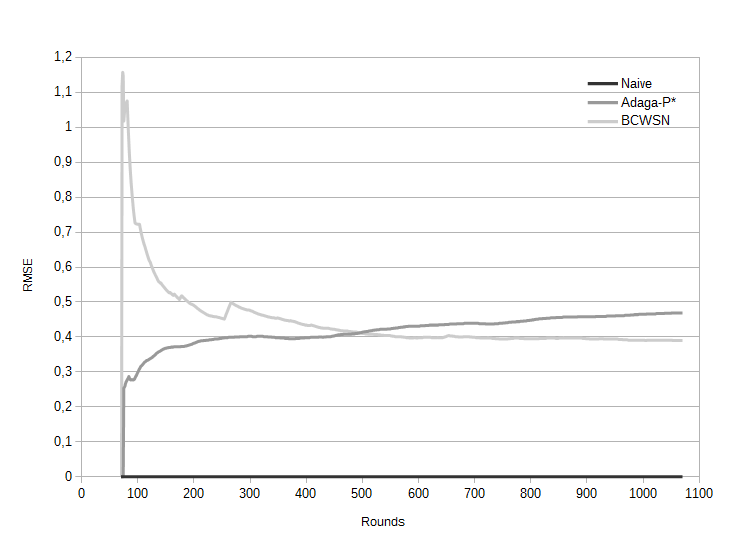
\includegraphics[scale=0.4]{BCWSN-RMSExRound-PB-Temp.png}
	 \vspace*{-.5cm}
	\caption{RMSE por rodada – Temperatura}
    %\caption{RMSE per round - Temperature}
    \label{fig:rmse}
\end{center}
\end{figure}
\vspace*{-.3cm}

Na Figura \ref{fig:rmse}, ele pode ser identificado uma pico na curva para o
BCWSN. A razão para isto é o fato de que o primeiro Cluster formado ter
é apenas uma etapa da inicialização para esta abordagem. Assim, a precisão 
BCWSN é comprometida no início. No entanto, a abordagem BCWSN é capaz de 
dinamicamente ajustar precisão através da redução do RMSE, através da 
utilização do Fractal Clustering (FC).
% In Figure \ref{fig:rmse}, it can be identified a peak for the BCWSN curve. The
% reason for this is the fact that the first cluster formation is only an
% initialization step for this approach. Thus, the BCWSN accuracy is jeopardized at
% the beginning. Nonetheless, BCWSN approach is able to dynamically adjust the
% accuracy by reducing the RMSE through the use of Fractal Clustering (FC).
\vspace*{-.3cm}

A Figura \ref{fig:num-msg} mostra o número de mensagens transmitidas por round.
Na abordagem Naive, o número de mensagens está constante, uma vez que
em cada rodada todos os sensores enviam dados coletados para a sink. 
No entanto, existem alguns picos na curva do BCWSN, as quais representam
períodos de tempo em que os clusters estão sendo reestruturadas 
(splitting or merging). {Lembrando que BCWSN dinamicamente atualiza a
configuração do clusters .}Essa característica de a abordagem proposta
é responsável pelo alto padrão desvio na Tabela \ref{tab:num-msg}.
% Figure \ref{fig:num-msg} depicts the number of transmitted messages per round.
% In the Naive approach, the number of messages is constant, since in each round
% all sensors send sensed data to the sink. Worth to be noted that, there are some
% peaks in BCWSN curve, which represent periods in time when clusters are being
% restructured (splitting or merging). {Recall that BCWSN dynamically updates the
% cluster configuration.} Such a characteristic of the proposed approach is
% responsible for the high standard deviation in Table \ref{tab:num-msg}.
\vspace*{-.3cm}
%{} = CanBeRemoved

\begin{figure}[!htb]
\begin{center}
	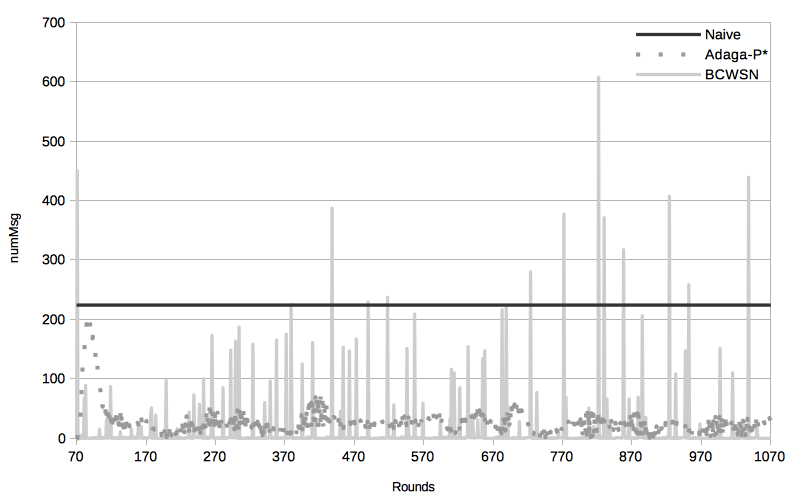
\includegraphics[scale=0.28]{BCWSN-NumMsgPerRoundxRound-PB-Temp.png}
	 \vspace*{-.6cm}
	 \caption{Mensagens por rodada – Temperatura} 
    %\caption{Messages per round - Temperature}
    \label{fig:num-msg}
\end{center}
\end{figure}
\vspace*{-.6cm}


Na Figura \ref{fig:tot-num-msg}, o número total de mensagens enviadas pelos
sensores em BCWSN é muito menor em comparação com Adaga-P *,
{ apesar de a grande variação no número de mensagens enviadas por rodada no
anterior (Figure \ref{fig:num-msg}).} 
% In Figure \ref{fig:tot-num-msg}, the total number of messages sent by sensors in
% BCWSN is much smaller compared to Adaga-P*{, despite the wide variation in the
% number of messages sent per round in the former (Figure \ref{fig:num-msg})}.
%{} = CanBeRemoved
\vspace*{-.3cm}

A Figura \ref{fig:num-clts} mostra a variação do número de clusters
a partir do BCWSN, que demonstra como a nossa proposta é capaz de se
adaptar a alterações no ambiente, assim mudando o clusters para refletir
essas mudanças.
% Figure \ref{fig:num-clts} shows the variation in the number of clusters from
% BCWSN that demonstrates how our proposal is able to adapt to changes in the
% sensed environment by changing the clusters to reflect such changes.
%\vspace*{-.3cm}
\vspace*{-.3cm}

\begin{figure}[!htb]
\begin{center}
	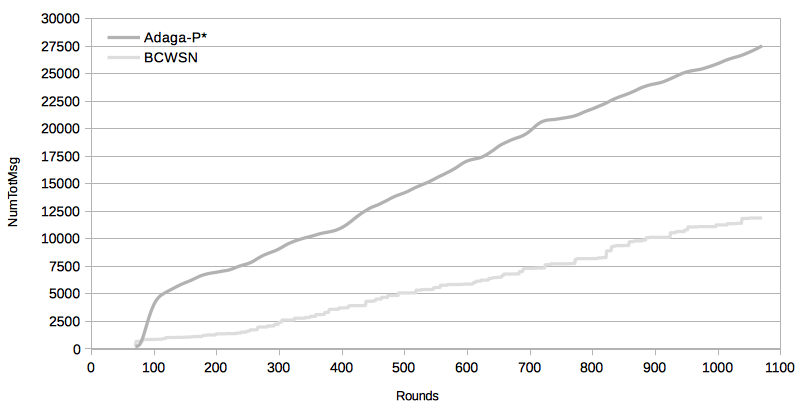
\includegraphics[scale=0.30]{BCWSN-TotNumMsgxRound-PB-Temp.png}
	 \vspace*{-.6cm}
	\caption{Número total de mensagens – Temperatura}
%     \caption{Total number of messages - Temperature}
    \label{fig:tot-num-msg}
\end{center}
\end{figure}
\vspace*{-.3cm}

\begin{figure}[!htb]
\begin{center}
	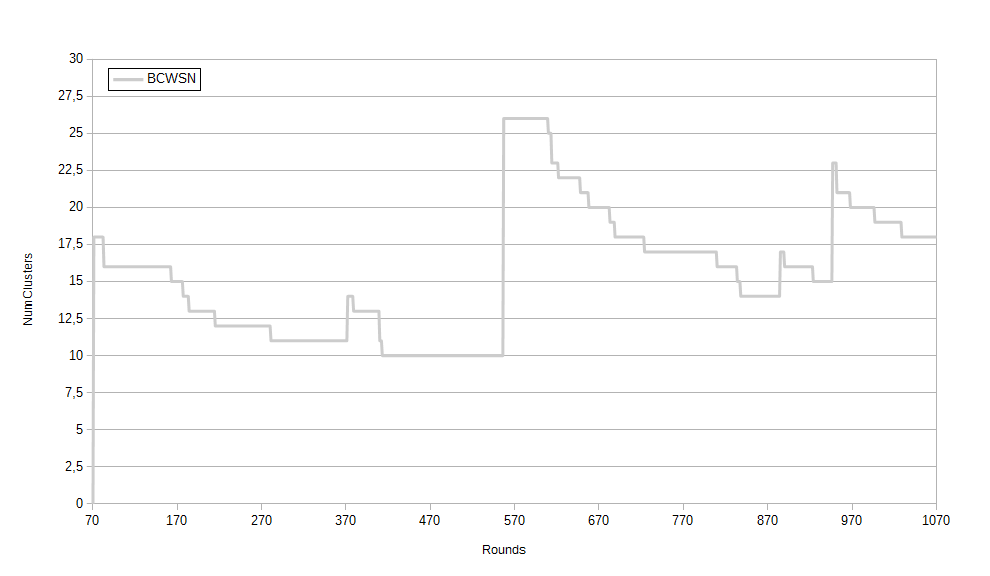
\includegraphics[scale=0.32]{BCWSN-NumClustersxRound-PB.png}
	 \vspace*{-.6cm}
	\caption{Número de clusters por rodada – Temperatura}
%     \caption{Number of clusters per round - Temperature}
    \label{fig:num-clts}
\end{center}
\end{figure}
%\vspace*{-.3cm}

Em seguida, apresentam-se os resultados do teste para {\ it umidade}, para mostrar a eficiência do 
abordagem proposta com outro sentiu tipo de dados.
% Next, we present the test results for {\it humidity}, to show the efficiency of the
% proposed approach with another sensed data type.
\vspace*{-.3cm}

\begin{figure}[!htb]
\begin{center}
	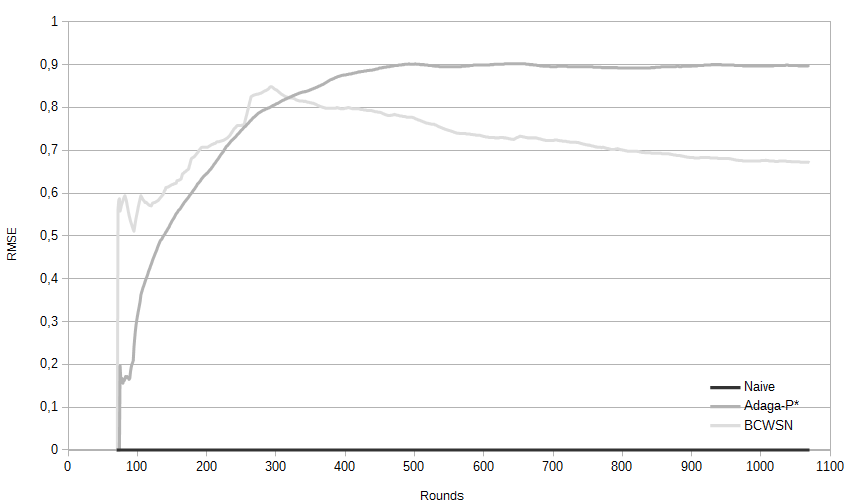
\includegraphics[scale=0.28]{BCWSN-RMSExRound-BW-Hum.png}
	 \vspace*{-.6cm}
	 \caption{RMSE por rodada – Umidade}
   % \caption{RMSE per round - Humidity}
    \label{fig:rmse-hum}
\end{center}
\end{figure}
% \vspace*{-.3cm}

A Figura \ref{fig:rmse-hum} mostra que, para a umidade, RMSE de BCWSN 
começa maior do que Adaga-P *. No entanto, a partir de um determinado ponto
(Ronda 320) em diante, ele cai, e fica inferior ao RMSE do Adaga-P *.
% Figure \ref{fig:rmse-hum} shows that, for humidity, BCWSN's RMSE starts higher
% than Adaga-P*. However, from a certain point in time (round 320) on, it drops
% lower than RMSE for Adaga-P*.
\vspace*{-.3cm}

Na Figura \ref{fig:tot-num-msg-hum}, pode-se compreender que o número total das mensagens no caso
de BCWSN é também menor do que a Adaga-P *. {Por uma questão de clareza,
não se incluiu a curva Naive para o número total de mensagens, porque ele
é muito alto w.r.t. as outras duas abordagens.}
% In Figure \ref{fig:tot-num-msg-hum}, it can be realized that the total number of
% messages in the case of BCWSN is also lower than the Adaga-P*. {For the sake of
% clarity, we did not included the Naive curve for the total number of messages,
% because it is too high w.r.t. the other two approaches.}
%\vspace*{-.3cm}
%{} = CanBeRemoved
\vspace*{-.3cm}

\begin{figure}[!htb]
\begin{center}
	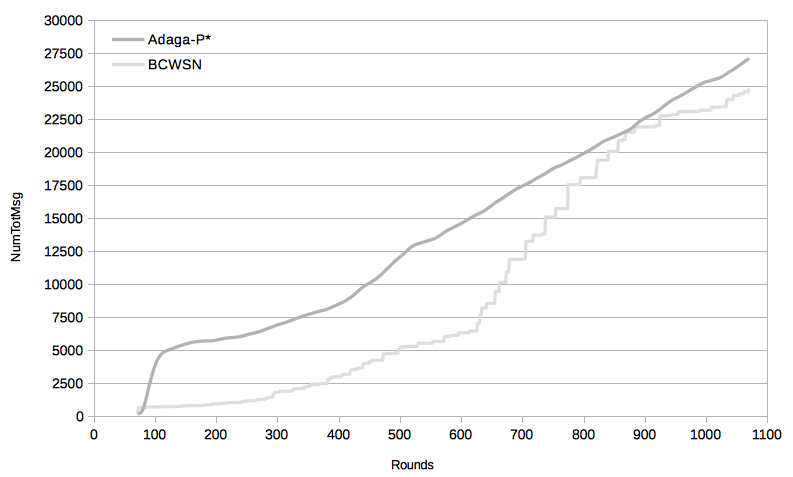
\includegraphics[scale=0.3]{BCWSN-TotNumMsgxRound-PB-Hum.png}
	 \vspace*{-.6cm}
    \caption{Número total de mensagens – Umidade}
    %\caption{Total number of messages - Humidity}
    \label{fig:tot-num-msg-hum}
\end{center}
\end{figure}
%\vspace*{-.3cm}

\section{Conclusion}
\label{conclusion}

Neste trabalho, foi descrita uma nova abordagem para o agrupamento
de sensores em RSSFs com base na noção de Behavioral Correlation e Fractal
Clustering. BCWSN identifica sensores com padrões de leitura 
de dados semelhantes, entre leituras de um ou mais (diferente) de tipos 
de dados. Desde Behavioral Correlation pode variar no tempo, BCWSN ajusta
dinamicamente a Behavioral Correlation a coleta de dados pelos nós sensores,
utilizando Fractal Clustering.
% In this paper, it was described a new approach for clustering sensors in WSNs
% based on the notion of Behavioral Correlation and Fractal Clustering.
% BCWSN identifies sensors with similar data reading patterns, among one or more
% (different) data type readings. Since behavioral correlation may vary in time,
% BCWSN dynamically adjusts the behavioral correlation among the data collect by
% the sensor nodes, using Fractal Clustering.
\vspace*{-.3cm}

Os resultados apresentados na Seção \ref{results-and-discussion} mostra 
BCWSN pode diminuir significativamente o consumo de energia em redes de
sensores, reduzindo o número total de mensagens transmitidas na rede (Figuras
\ref{fig:tot-num-msg} e \ref{fig:tot-num-msg-hum}),garantindo ao mesmo
tempo um baixo erro RMS. Os resultados apresentados nas tabelas \ref{tab:rmse} 
e \ref{tab:num-msg} mostra esta afirmação, uma vez que o consumo de 
energia (para o envio de mensagens) na Adaga-P * foi de $2.33$ vezes maior do
que a energia consumida  para executar BCWSN para recolha de temperatura 
(em $1000$ ciclos, com limiar de $5\%$), por uma diferença RMSE de $0.026$.
% The results presented in Section \ref{results-and-discussion} show BCWSN may
% significantly decrease energy consumption in WSNs, by reducing the total number
% of messages transmitted in the network (Figures \ref{fig:tot-num-msg} and
% \ref{fig:tot-num-msg-hum}), while assuring a low RMS Error. The results
% presented in Tables \ref{tab:rmse} and \ref{tab:num-msg} proves this assertion,
% since energy consumption (for sending messages) in Adaga-P* was $2.33$ times
% higher than the energy consumed to execute BCWSN for gathering {\it temperature}
% (in $1000$ cycles, with threshold of $5\%$), for a RMSE difference of $0.026$.
\vspace*{-.6cm}

Por fim, enfatizamos a aplicabilidade e a eficácia da BCWSN para uma variedade de aplicações que
consomem dados produzidos por redes de sensores.
% Finally, we emphasize the applicability and the effectiveness of BCWSN for a
% variety of applications which consume data produced by WSNs.
%\vspace*{-.3cm}
\vspace*{-.3cm}

%Currently, we are working on
%measuring distance between prediction models to assess the dissimilarity in
%sensed data behavior. Moreover, we are evaluating the use of traditional
%techniques of data mining, such as K-Means, to perform the initial grouping of
%sensors into clusters, overriding the use of similarity measures for such
%purpose.



\bibliographystyle{abbrv}
\bibliography{Artigo_SAC}  
% SAC2015rodrigues_brayner_maia.bib is the name of the Bibliography in this case
% You must have a proper ".bib" file
%  and remember to run:
% latex bibtex latex latex
% to resolve all references

\end{document}